% ============================================================
% CHƯƠNG 3 — THIẾT KẾ, TRIỂN KHAI VÀ ĐÁNH GIÁ HỆ THỐNG  (mẫu SoICT chương 4)
% Sắp xếp lại ngày 07/11/2026 theo mẫu Do_An_Latex_SoiCT: gộp Chương 3 cũ (Phân tích và thiết kế),
% Chương 4 cũ (Xây dựng hệ thống) và Chương 5 cũ (Kết quả thực nghiệm). Bản trước:
% backup/2026-11-07_truoc-mau-soict/Chap3.tex, Chap4.tex, Chap5.tex.
% Phần phân tích yêu cầu (tác nhân, use case, yêu cầu chức năng, phi chức năng) đã chuyển lên Chương 1
% (mục Khảo sát hiện trạng, Tổng quan chức năng, Đặc tả chức năng, Yêu cầu phi chức năng).
%
% Bố cục theo mẫu SoICT: Thiết kế kiến trúc (lựa chọn kiến trúc, thiết kế tổng quan = biểu đồ gói,
% thiết kế chi tiết gói) -> Thiết kế chi tiết (giao diện, lớp + biểu đồ trình tự, CSDL) -> Xây dựng ứng dụng
% (thư viện và công cụ có phiên bản, kết quả đạt được có thống kê mã nguồn, minh họa chức năng chính)
% -> Kiểm thử (2–3 chức năng quan trọng, kỹ thuật kiểm thử, tổng kết) -> Triển khai.
% Theo mẫu, nội dung là đóng góp chính chỉ tóm lược ở đây và tham chiếu sang Chương 4
% ("Chi tiết được trình bày ở mục~\ref{...}"), không trình bày lặp lại.
% Văn phong: xem ghi chú đầu Chap1.tex (hạn chế xưng "em"; mục con dùng \subsection*, không \ref tới mục con). [BẢN NHÁP] Sinh viên đọc lại và sửa theo văn phong của mình.
% ============================================================

\chapter{THIẾT KẾ, TRIỂN KHAI VÀ ĐÁNH GIÁ HỆ THỐNG}
\chaptermark{THIẾT KẾ, TRIỂN KHAI VÀ ĐÁNH GIÁ}
\label{chap:thietke}
\label{chap:xaydung}
\label{chap:ketqua}
% ============================================================
% HÌNH VẼ CHƯƠNG 3 (TikZ) — gọi bằng macro trong Chap3.tex
%   \HinhUseCase     : biểu đồ ca sử dụng tổng quát        (fig:usecase)
%   \HinhOnOffChain  : phân tách dữ liệu on/off-chain       (fig:onoffchain)
%   \HinhTrangThai   : biểu đồ trạng thái của lô tín chỉ    (fig:trangthai)
% Đây là bản đề xuất theo phiếu giao nhiệm vụ: sửa lại cho khớp thiết kế thực tế của bạn.
% ============================================================

% Hình người (tác nhân UML)
\tikzset{
  tacnhan/.pic={
    \draw[thick] (0,0.62) circle (0.15);
    \draw[thick] (0,0.47) -- (0,0.05);
    \draw[thick] (-0.25,0.33) -- (0.25,0.33);
    \draw[thick] (0,0.05) -- (-0.18,-0.28);
    \draw[thick] (0,0.05) -- (0.18,-0.28);
  }
}

% ---------- Biểu đồ ca sử dụng tổng quát ----------
\newcommand{\HinhUseCase}{%
\begin{figure}[htbp]
\centering
\begin{tikzpicture}[font=\footnotesize]
  % Khung hệ thống
  % Sửa ngày 07/11/2026: VVB thẩm định, phê duyệt; cơ quan quản lý phát hành (mint).
  \draw[thick] (3.0,-5.2) rectangle (9.8,4.6);
  \node[font=\footnotesize\bfseries] at (6.4,4.25) {Hệ thống quản lý tín chỉ các-bon};
  % Ca sử dụng: tên nút / tung độ / nội dung
  \foreach \ten/\y/\noidung in {
      uc1/3.5/{Thẩm định, phê duyệt yêu cầu cấp},
      uc2/2.6/{Đăng ký dự án},
      uc3/1.7/{Gửi yêu cầu cấp tín chỉ},
      uc4/0.8/{Nạp tín chỉ vào pool, đổi token},
      uc5/-0.1/{Mua bán, chuyển nhượng tín chỉ},
      uc6/-1.0/{Hủy tín chỉ để bù trừ (retire)},
      uc7/-1.9/{Tra cứu tín chỉ, chứng nhận hủy},
      uc8/-2.8/{Theo dõi dashboard hạn ngạch},
      uc9/-3.7/{Quản lý tài khoản, phân quyền},
      uc10/-4.6/{Phát hành lô tín chỉ (mint)}} {
    \draw (6.4,\y) ellipse (3.2cm and 0.38cm);
    \node at (6.4,\y) {\noidung};
    \coordinate (\ten-w) at (3.2,\y);
    \coordinate (\ten-e) at (9.6,\y);
  }
  % Tác nhân bên trái (tên ở dưới)
  \pic at (1.2,3.1) {tacnhan};   \node[align=center] at (1.2,2.55) {VVB};
  \pic at (1.2,0.8) {tacnhan};   \node[align=center] at (1.2,0.25) {Chủ dự án};
  % Tác nhân bên phải (tên ở bên phải để không đè lên đường nối)
  \pic at (11.2,0.5) {tacnhan};  \node[align=left, anchor=west] at (11.5,0.55) {Doanh nghiệp\\mua};
  \pic at (11.2,-3.0) {tacnhan}; \node[align=left, anchor=west] at (11.5,-2.95) {Cơ quan\\quản lý};
  % Liên kết
  \draw (1.5,3.4) -- (uc1-w);
  \foreach \u in {uc2,uc3,uc4,uc5} \draw (1.5,1.1) -- (\u-w);
  \foreach \u in {uc4,uc5,uc6,uc7} \draw (10.9,0.8) -- (\u-e);
  \foreach \u in {uc7,uc8,uc9,uc10} \draw (10.9,-2.7) -- (\u-e);
\end{tikzpicture}
\caption[Biểu đồ ca sử dụng tổng quát của hệ thống]{Biểu đồ ca sử dụng tổng quát của hệ thống \hinhtao[Claude]{20/10/2026; Updated: 07/11/2026}}
\label{fig:usecase}
\end{figure}}

% ---------- Phân tách dữ liệu on-chain / off-chain ----------
\newcommand{\HinhOnOffChain}{%
\begin{figure}[htbp]
\centering
\begin{tikzpicture}[
    >=Stealth,
    o/.style={draw, rounded corners=2pt, align=left, font=\footnotesize,
              text width=4.7cm, inner sep=4pt, fill=white},
    nhan/.style={font=\scriptsize, align=center, text width=2.6cm}]
  % Off-chain
  \node[o] (files) at (2.6,1.6) {\textbf{Kho tệp}\\
      IPFS hoặc lưu trữ đối tượng:\\
      PDD, báo cáo thẩm định,\\ tệp metadata JSON};
  \node[o, below=5mm of files] (db) {\textbf{CSDL quan hệ}\\
      PostgreSQL, theo mô hình\\ CAD Trust V2.0:\\
      Project, Stakeholders,\\ Verifications, Issuances, Units;\\
      tài khoản ứng dụng (bảng riêng);\\
      lịch sử giao dịch đồng bộ từ sự kiện};
  \node[draw, thick, dashed, rounded corners=4pt, inner sep=6pt, fit=(files)(db),
        label={[font=\footnotesize\bfseries]above:Off-chain (backend)}] (off) {};
  % On-chain
  \node[o, fill=gray!10] (nft) at (11.0,1.6) {\textbf{Hợp đồng NFT tín chỉ (ERC-721)}\\
      tokenId, chủ sở hữu, số sê-ri,\\ mã băm hồ sơ, URI metadata};
  \node[o, fill=gray!10, below=4mm of nft] (pool) {\textbf{Hợp đồng pool (ERC-20)}\\
      số dư token,\\ NFT đang khóa trong pool};
  \node[o, fill=gray!10, below=4mm of pool] (ret) {\textbf{Module Retirement}\\
      sự kiện Retired, người thụ hưởng};
  \node[draw, thick, rounded corners=4pt, inner sep=6pt, fit=(nft)(pool)(ret),
        label={[font=\footnotesize\bfseries]above:On-chain (Ethereum Sepolia)}] (on) {};
  % Luồng dữ liệu
  \draw[->, thick] (files.east) -- node[nhan, above] {mã băm hồ sơ (keccak256) và URI khi mint}
      (on.west |- files.east);
  \draw[->, thick] (on.west |- db.east) -- node[nhan, below] {sự kiện Minted, Transfer, Retired: backend đồng bộ}
      (db.east);
\end{tikzpicture}
\caption[Phân tách dữ liệu giữa phần on-chain và off-chain của hệ thống]{Phân tách dữ liệu giữa phần on-chain và off-chain của hệ thống \hinhtao[Claude]{20/10/2026}}
\label{fig:onoffchain}
\end{figure}}

% ---------- Biểu đồ trạng thái của một lô tín chỉ ----------
\newcommand{\HinhTrangThai}{%
\begin{figure}[htbp]
\centering
\begin{tikzpicture}[
    >=Stealth,
    tt/.style={draw, rounded corners=6pt, align=center, font=\footnotesize,
               minimum height=0.9cm, inner xsep=5pt, fill=white},
    nhan/.style={font=\scriptsize, align=center}]
  \node[circle, fill=black, inner sep=3pt] (bd) at (0,0) {};
  \node[tt] (nhap)   at (1.4,0)   {Nháp};
  \node[tt] (cho)    at (4.5,0)   {Chờ thẩm định};
  \node[tt] (tuchoi) at (4.5,-2.3) {Bị từ chối};
  \node[tt] (dacap)  at (9.0,0)   {Đã cấp\\(NFT ERC-721)};
  \node[tt] (pool)   at (9.0,-2.6) {Trong pool\\(ERC-20)};
  \node[tt] (dahuy)  at (12.6,0)   {Đã hủy\\(retired)};
  \node[circle, draw, inner sep=4pt] (kt) at (14.1,0) {};
  \node[circle, fill=black, inner sep=2pt] at (kt) {};

  \draw[->] (bd) -- (nhap);
  \draw[->] (nhap) -- node[nhan, above] {gửi\\hồ sơ} (cho);
  \draw[->] (cho) -- node[nhan, above] {VVB duyệt; cơ quan\\quản lý mint NFT} (dacap);
  \draw[->] (cho) -- node[nhan, right] {VVB từ chối} (tuchoi);
  \draw[->] (tuchoi.west) -| node[nhan, pos=0.3, below] {bổ sung hồ sơ} (nhap.south);
  \draw[->] (dacap) -- node[nhan, above] {hủy hết\\(burn NFT)} (dahuy);
  \draw[->] (dahuy) -- (kt);
  \draw[->] ([xshift=-5mm]dacap.south) -- node[nhan, left] {nạp vào pool} ([xshift=-5mm]pool.north);
  \draw[->] ([xshift=5mm]pool.north) -- node[nhan, right] {đổi lại\\(redeem)} ([xshift=5mm]dacap.south);
  \draw[->] (pool.east) -| node[nhan, pos=0.3, below] {hủy hết phần còn lại\\ từ pool} (dahuy.south);
  \draw[->] ([xshift=-4mm]dacap.north) .. controls +(-0.3,0.9) and +(0.3,0.9) ..
      node[nhan, above] {chuyển nhượng; hủy một phần} ([xshift=4mm]dacap.north);
  \draw[->] ([xshift=-4mm]pool.south) .. controls +(-0.3,-0.9) and +(0.3,-0.9) ..
      node[nhan, below] {giao dịch token PCC; hủy một phần} ([xshift=4mm]pool.south);
\end{tikzpicture}
\caption[Biểu đồ trạng thái của một lô tín chỉ các-bon trong hệ thống]{Biểu đồ trạng thái của một lô tín chỉ các-bon trong hệ thống \hinhtao[Claude]{20/10/2026; Updated: 07/11/2026}}
\label{fig:trangthai}
\end{figure}}

% ============================================================
% HÌNH BỔ SUNG GIAI ĐOẠN 3–4 (vẽ theo mã nguồn thực tế trong contracts/ và backend/)
%   \HinhLopHopDong   : biểu đồ lớp các hợp đồng thông minh   (fig:lophopdong)
%   \HinhERD          : lược đồ CSDL off-chain                 (fig:erd)
%   \HinhTuanTuMint   : tuần tự yêu cầu cấp – thẩm định – mint (fig:tuantu-mint)
%   \HinhTuanTuRetire : tuần tự nạp pool – giao dịch – hủy     (fig:tuantu-retire)
%   \BangAPI          : bảng endpoint API REST                 (tab:api)
% ============================================================

% Hộp lớp UML: tên / thuộc tính / phương thức
\newcommand{\lopUML}[3]{%
  \begin{tabular}{@{}l@{}}
    \multicolumn{1}{c}{\textbf{#1}}\\ \hline
    \rule{0pt}{2.4ex}#2\\ \hline
    \rule{0pt}{2.4ex}#3
  \end{tabular}}

\newcommand{\HinhLopHopDong}{%
\begin{figure}[htbp]
\centering
\begin{adjustbox}{max width=\textwidth}
\begin{tikzpicture}[
    >=Stealth, font=\scriptsize,
    lop/.style={draw, fill=white, inner sep=3pt, align=left},
    oz/.style={draw, dashed, rounded corners=2pt, inner sep=3pt, font=\scriptsize\itshape, fill=gray!8},
    ke/.style={-{Triangle[open]}, thick},
    dung/.style={->, dashed}]
  % Thư viện OpenZeppelin
  \node[oz] (erc721) at (0.2,4.8) {ERC721URIStorage};
  \node[oz] (ac)     at (3.0,4.8) {AccessControl};
  \node[oz] (pa)     at (5.4,4.8) {Pausable};
  \node[oz] (erc20)  at (9.8,4.8) {ERC20};
  \node[oz] (recv)   at (12.2,4.8) {IERC721Receiver};
  \node[oz] (rg)     at (15.0,4.8) {ReentrancyGuard};

  \node[lop, anchor=north] (nft) at (2.8,3.8) {\lopUML{CarbonCreditNFT}{%
      + ISSUER\_ROLE, RETIREMENT\_AGENT\_ROLE : bytes32\\
      - \_batches : mapping(uint256 $\Rightarrow$ CreditBatch)\\
      - \_certificates : RetirementCertificate[]\\
      + nextAvailableSerial : mapping(bytes32 $\Rightarrow$ uint256)\\
      + documentUsed : mapping(bytes32 $\Rightarrow$ bool)}{%
      + mintBatch(to, projectId, vintage, serialFrom, quantity,\\
      \quad documentHash, uri) : uint256 \quad \textit{onlyRole(ISSUER)}\\
      + retire(tokenId, amount, beneficiary, reason) : uint256\\
      + retireFor(retiree, tokenId, amount, beneficiary, reason)\\
      \quad \textit{onlyRole(RETIREMENT\_AGENT)}\\
      + pause(), unpause() \quad \textit{onlyRole(DEFAULT\_ADMIN)}\\
      + getBatch(tokenId), remainingOf(tokenId), getCertificate(id)\\
      \textit{sự kiện:} CreditMinted, CreditRetired}};

  \node[lop, anchor=north] (pool) at (12.4,3.8) {\lopUML{CarbonPool}{%
      + credits : CarbonCreditNFT \quad \textit{immutable}\\
      - \_pooled : EnumerableSet.UintSet\\
      + decimals() = 0 \quad (1 PCC = 1 tCO$_2$e)}{%
      + deposit(tokenId)\\
      + onERC721Received(...) : đúc PCC cho người nạp\\
      + redeem(tokenId) : đốt PCC, trả NFT\\
      + retire(tokenId, amount, beneficiary, reason)\\
      + pooledTokenIds(), isPooled(tokenId)\\
      \textit{sự kiện:} Deposited, Redeemed, RetiredFromPool}};

  \node[lop, anchor=north] (batch) at (2.8,-2.6) {\lopUML{$\ll$struct$\gg$ CreditBatch}{%
      projectId : string; vintage : uint16\\
      serialFrom, quantity, retired : uint256\\
      documentHash : bytes32; issuer : address\\
      issuedAt : uint64}{\textit{(dữ liệu của một lô)}}};

  \node[lop, anchor=north] (cert) at (12.4,-1.4) {\lopUML{$\ll$struct$\gg$ RetirementCertificate}{%
      tokenId, serialFrom, serialTo, amount : uint256\\
      retiree : address\\
      beneficiary, reason : string; retiredAt : uint64}{\textit{(một chứng nhận hủy)}}};

  \draw[ke] ([xshift=-2.6cm]nft.north) -- (erc721.south);
  \draw[ke] ([xshift=0.2cm]nft.north) -- (ac.south);
  \draw[ke] ([xshift=2.6cm]nft.north) -- (pa.south);
  \draw[ke] ([xshift=-2.6cm]pool.north) -- (erc20.south);
  \draw[ke] ([xshift=-0.2cm]pool.north) -- (recv.south);
  \draw[ke] ([xshift=2.6cm]pool.north) -- (rg.south);
  \draw[dung] (pool.west) -- node[above, align=center] {gọi retireFor,\\ safeTransferFrom} (nft.east |- pool.west);
  \draw[-{Diamond[open]}] (batch.north) -- (nft.south);
  \draw[-{Diamond[open]}] (cert.west) -- ++(-1.2,0) |- ([yshift=4mm]nft.south east);
\end{tikzpicture}
\end{adjustbox}
\caption[Biểu đồ lớp của các hợp đồng thông minh]{Biểu đồ lớp của các hợp đồng thông minh \hinhtao[Claude]{21/10/2026; Updated: 07/11/2026}}
\label{fig:lophopdong}
\end{figure}}

% ---------- Lược đồ CSDL ----------
% Bảng ERD: tên bảng / danh sách cột (khóa chính in đậm, khóa ngoại in nghiêng)
\newcommand{\bangERD}[2]{%
  \begin{tabular}{@{}l@{}}
    \multicolumn{1}{c}{\textbf{#1}}\\ \hline
    \rule{0pt}{2.2ex}#2
  \end{tabular}}

\newcommand{\HinhERD}{%
\begin{figure}[htbp]
\centering
\begin{adjustbox}{max width=\textwidth}
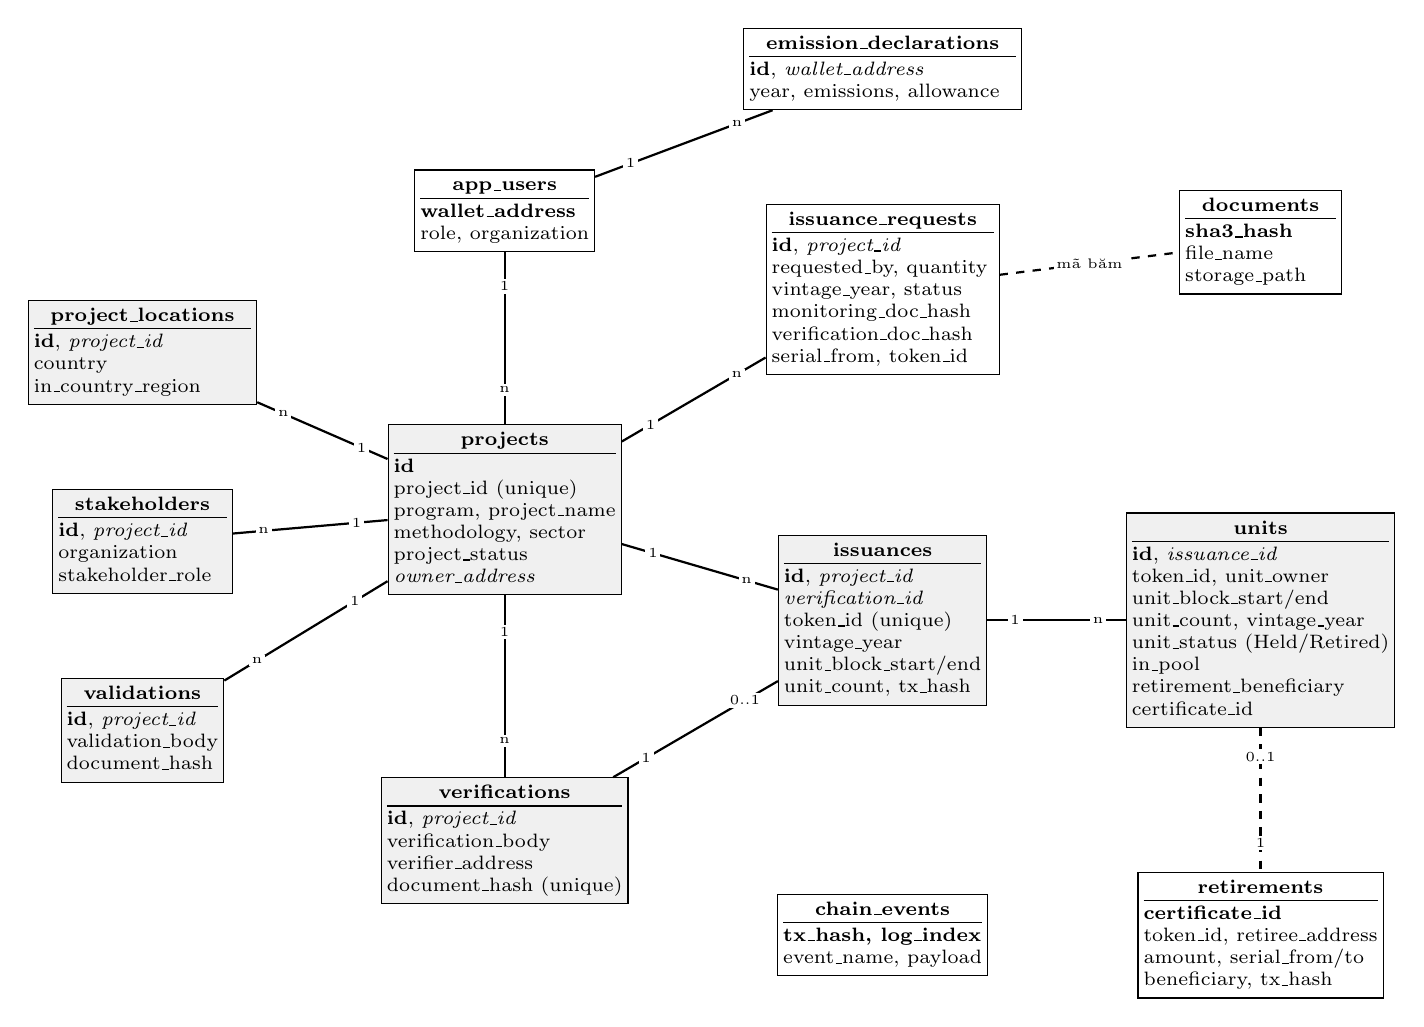
\begin{tikzpicture}[font=\scriptsize,
    bang/.style={draw, fill=white, inner sep=2pt, align=left},
    cad/.style={bang, fill=gray!12},
    lk/.style={draw, thick},
    n/.style={font=\tiny, fill=white, inner sep=1pt}]
  % Nhóm CAD Trust (nền xám)
  \node[cad] (proj) at (0,0) {\bangERD{projects}{%
     \textbf{id}\\ project\_id (unique)\\ program, project\_name\\ methodology, sector\\
     project\_status\\ \textit{owner\_address}}};
  \node[cad] (loc) at (-4.6,2.0) {\bangERD{project\_locations}{\textbf{id}, \textit{project\_id}\\ country\\ in\_country\_region}};
  \node[cad] (sh)  at (-4.6,-0.4) {\bangERD{stakeholders}{\textbf{id}, \textit{project\_id}\\ organization\\ stakeholder\_role}};
  \node[cad] (val) at (-4.6,-2.8) {\bangERD{validations}{\textbf{id}, \textit{project\_id}\\ validation\_body\\ document\_hash}};
  \node[cad] (ver) at (0,-4.2) {\bangERD{verifications}{\textbf{id}, \textit{project\_id}\\ verification\_body\\ verifier\_address\\ document\_hash (unique)}};
  \node[cad] (iss) at (4.8,-1.4) {\bangERD{issuances}{\textbf{id}, \textit{project\_id}\\ \textit{verification\_id}\\ token\_id (unique)\\ vintage\_year\\ unit\_block\_start/end\\ unit\_count, tx\_hash}};
  \node[cad] (unit) at (9.6,-1.4) {\bangERD{units}{\textbf{id}, \textit{issuance\_id}\\ token\_id, unit\_owner\\ unit\_block\_start/end\\ unit\_count, vintage\_year\\ unit\_status (Held/Retired)\\ in\_pool\\ retirement\_beneficiary\\ certificate\_id}};
  % Nhóm riêng của ứng dụng (nền trắng)
  \node[bang] (user) at (0,3.8) {\bangERD{app\_users}{\textbf{wallet\_address}\\ role, organization}};
  \node[bang] (req)  at (4.8,2.8) {\bangERD{issuance\_requests}{\textbf{id}, \textit{project\_id}\\ requested\_by, quantity\\ vintage\_year, status\\ monitoring\_doc\_hash\\ verification\_doc\_hash\\ serial\_from, token\_id}};
  \node[bang] (doc)  at (9.6,3.4) {\bangERD{documents}{\textbf{sha3\_hash}\\ file\_name\\ storage\_path}};
  \node[bang] (ret)  at (9.6,-5.4) {\bangERD{retirements}{\textbf{certificate\_id}\\ token\_id, retiree\_address\\ amount, serial\_from/to\\ beneficiary, tx\_hash}};
  \node[bang] (emi)  at (4.8,5.6) {\bangERD{emission\_declarations}{\textbf{id}, \textit{wallet\_address}\\ year, emissions, allowance}};
  \node[bang] (evt)  at (4.8,-5.4) {\bangERD{chain\_events}{\textbf{tx\_hash, log\_index}\\ event\_name, payload}};

  \draw[lk] (proj) -- node[n, pos=0.2]{1} node[n, pos=0.8]{n} (loc);
  \draw[lk] (proj) -- node[n, pos=0.2]{1} node[n, pos=0.8]{n} (sh);
  \draw[lk] (proj) -- node[n, pos=0.2]{1} node[n, pos=0.8]{n} (val);
  \draw[lk] (proj) -- node[n, pos=0.2]{1} node[n, pos=0.8]{n} (ver);
  \draw[lk] (proj) -- node[n, pos=0.2]{1} node[n, pos=0.8]{n} (iss);
  \draw[lk] (ver) -- node[n, pos=0.2]{1} node[n, pos=0.8]{0..1} (iss);
  \draw[lk] (iss) -- node[n, pos=0.2]{1} node[n, pos=0.8]{n} (unit);
  \draw[lk] (user) -- node[n, pos=0.2]{1} node[n, pos=0.8]{n} (proj);
  \draw[lk] (proj) -- node[n, pos=0.2]{1} node[n, pos=0.8]{n} (req);
  \draw[lk] (user) -- node[n, pos=0.2]{1} node[n, pos=0.8]{n} (emi);
  \draw[lk, dashed] (unit) -- node[n, pos=0.2]{0..1} node[n, pos=0.8]{1} (ret);
  \draw[lk, dashed] (req) -- node[n]{mã băm} (doc);
\end{tikzpicture}
\end{adjustbox}
\caption[Lược đồ cơ sở dữ liệu off-chain (nền xám: các bảng theo mô hình CAD Trust V2.0)]{Lược đồ cơ sở dữ liệu off-chain (nền xám: các bảng theo mô hình CAD Trust V2.0) \hinhtao[Claude]{21/10/2026}}
\label{fig:erd}
\end{figure}}

% ---------- Biểu đồ tuần tự ----------
% \dongdoi{tên nút}{x}{nhãn}{y cuối}: vẽ một đường đời (lifeline)
\newcommand{\dongdoi}[4]{%
  \node[draw, fill=white, minimum width=1.9cm, minimum height=0.7cm, align=center, font=\scriptsize] (#1) at (#2,0) {#3};
  \draw[dashed, gray] (#1.south) -- (#2,#4);}
% \tinnhan[kiểu mũi tên]{x1}{x2}{y}{nhãn}
\newcommand{\tinnhan}[5][->]{%
  \draw[#1, >=Stealth] (#2,#4) -- node[above, font=\scriptsize, align=center] {#5} (#3,#4);}

\newcommand{\HinhTuanTuMint}{%
\begin{figure}[htbp]
\centering
\begin{adjustbox}{max width=\textwidth}
\begin{tikzpicture}[yscale=1.2]
  % Sửa ngày 07/11/2026: VVB chỉ phê duyệt; cơ quan quản lý ký giao dịch phát hành (mint).
  \dongdoi{cda}{0}{Chủ dự án\\(trình duyệt)}{-12.0}
  \dongdoi{be}{3.8}{Backend API}{-12.0}
  \dongdoi{db}{6.6}{PostgreSQL}{-12.0}
  \dongdoi{vvb}{9.4}{VVB\\(trình duyệt)}{-12.0}
  \dongdoi{cq}{12.4}{Cơ quan quản lý\\(MetaMask)}{-12.0}
  \dongdoi{sc}{15.4}{CarbonCreditNFT}{-12.0}
  \dongdoi{ix}{18.4}{Bộ đồng bộ\\sự kiện}{-12.0}
  \tinnhan{0}{3.8}{-1.2}{POST /documents (báo cáo giám sát)}
  \tinnhan[<-]{0}{3.8}{-1.8}{sha3\_hash}
  \tinnhan{0}{3.8}{-2.5}{POST /issuance-requests}
  \tinnhan{3.8}{6.6}{-3.0}{INSERT, status = SUBMITTED}
  \tinnhan[<-]{3.8}{9.4}{-3.8}{GET /issuance-requests (danh sách chờ)}
  \tinnhan[<-]{3.8}{9.4}{-4.5}{POST /documents (báo cáo thẩm định)}
  \tinnhan[<-]{3.8}{9.4}{-5.2}{POST /issuance-requests/:id/approve}
  \tinnhan{3.8}{6.6}{-6.1}{kiểm tra mã băm chưa dùng;\\ INSERT verifications; APPROVED}
  \tinnhan[<-]{3.8}{12.4}{-6.9}{GET /issuance-requests (đã phê duyệt)}
  \tinnhan{3.8}{12.4}{-7.8}{tham số mint (to, projectId, vintage,\\ serialFrom, quantity, documentHash, uri)}
  \tinnhan{12.4}{15.4}{-8.5}{mintBatch(...) ký bằng ví\\ cơ quan quản lý}
  \node[draw, fill=white, font=\scriptsize, align=left, anchor=west] at (15.55,-9.2) {kiểm tra ISSUER\_ROLE,\\ sê-ri không chồng lấn,\\ documentHash chưa dùng};
  \tinnhan{15.4}{18.4}{-10.3}{sự kiện CreditMinted, Transfer}
  \draw[->, >=Stealth] (18.4,-10.9) -- node[above, font=\scriptsize, align=center, pos=0.3] {INSERT issuances, units (Held); yêu cầu $\rightarrow$ MINTED} (6.6,-10.9);
  \tinnhan[<-]{0}{3.8}{-11.5}{trạng thái MINTED, lô \#tokenId}
\end{tikzpicture}
\end{adjustbox}
\caption[Biểu đồ tuần tự quy trình yêu cầu cấp, thẩm định và phát hành tín chỉ]{Biểu đồ tuần tự quy trình yêu cầu cấp, thẩm định và phát hành tín chỉ \hinhtao[Claude]{21/10/2026; Updated: 07/11/2026}}
\label{fig:tuantu-mint}
\end{figure}}

\newcommand{\HinhTuanTuRetire}{%
\begin{figure}[htbp]
\centering
\begin{adjustbox}{max width=\textwidth}
\begin{tikzpicture}[yscale=1.2]
  \dongdoi{cda}{0}{Chủ dự án\\(MetaMask)}{-9.4}
  \dongdoi{dn}{3.4}{Doanh nghiệp\\(MetaMask)}{-9.4}
  \dongdoi{pool}{7.0}{CarbonPool\\(ERC-20)}{-9.4}
  \dongdoi{nft}{10.6}{CarbonCreditNFT\\(ERC-721)}{-9.4}
  \dongdoi{ix}{14.2}{Bộ đồng bộ\\+ CSDL}{-9.4}
  \tinnhan{0}{10.6}{-1.2}{safeTransferFrom(chủ dự án, pool, tokenId)}
  \tinnhan[<-]{7.0}{10.6}{-1.9}{onERC721Received(from, tokenId)}
  \node[draw, fill=white, font=\scriptsize, align=left, anchor=east] at (6.85,-2.6) {\_mint(from, remainingOf(tokenId));\\ NFT bị khóa trong pool};
  \tinnhan{0}{7.0}{-3.6}{transfer(doanh nghiệp, 300): bán từng phần}
  \tinnhan{3.4}{7.0}{-4.5}{retire(tokenId, 300, ...)}
  \node[draw, fill=white, font=\scriptsize, align=left, anchor=east] at (6.85,-5.1) {\_burn(doanh nghiệp, 300)};
  \tinnhan{7.0}{10.6}{-5.8}{retireFor(doanh nghiệp, tokenId, 300, ...)}
  \node[draw, fill=white, font=\scriptsize, align=left, anchor=west] at (10.75,-6.6) {retired += 300; lưu chứng nhận\\ (sê-ri, người hủy, thụ hưởng);\\ hủy hết thì \_burn(tokenId)};
  \tinnhan{10.6}{14.2}{-7.9}{sự kiện CreditRetired, Transfer}
  \tinnhan[<-]{3.4}{14.2}{-8.6}{GET /api/retirements/:id: chứng nhận hủy công khai}
\end{tikzpicture}
\end{adjustbox}
\caption[Biểu đồ tuần tự giao dịch qua pool và hủy tín chỉ]{Biểu đồ tuần tự giao dịch qua pool và hủy tín chỉ \hinhtao[Claude]{21/10/2026}}
\label{fig:tuantu-retire}
\end{figure}}

% ---------- Bảng API ----------
\newcommand{\BangAPI}{%
\begingroup\small
\renewcommand{\arraystretch}{1.15}
\begin{longtable}{|p{1.35cm}|>{\footnotesize}p{5.6cm}|>{\footnotesize\raggedright\arraybackslash}p{2.3cm}|>{\raggedright\arraybackslash}p{3.9cm}|}
\caption{Các endpoint của API REST}\label{tab:api}\\
\hline
\textbf{HTTP} & \textbf{Đường dẫn} & \textbf{Quyền} & \textbf{Chức năng}\\ \hline
\endfirsthead
\hline
\textbf{HTTP} & \textbf{Đường dẫn} & \textbf{Quyền} & \textbf{Chức năng}\\ \hline
\endhead
POST & /api/auth/nonce & Công khai & Lấy thông điệp đăng nhập cần ký\\ \hline
POST & /api/auth/login & Công khai & Xác minh chữ ký ví, cấp JWT; tạo tài khoản lần đầu\\ \hline
GET & /api/auth/me & Đã đăng nhập & Thông tin tài khoản\\ \hline
GET & /api/users & ADMIN & Danh sách tài khoản\\ \hline
PATCH & /api/users/:address/role & ADMIN & Đổi vai trò\\ \hline
GET & /api/projects & Công khai & Danh sách dự án kèm tổng đã cấp, đã hủy\\ \hline
GET & /api/projects/:id & Công khai & Chi tiết dự án, vị trí, các bên, thẩm định, đợt cấp\\ \hline
POST & /api/projects & PROJECT\_\allowbreak OWNER & Đăng ký dự án\\ \hline
PATCH & /api/projects/:id & Chủ dự án, ADMIN & Sửa thông tin; ADMIN đổi trạng thái\\ \hline
POST & /api/documents & Đã đăng nhập & Tải hồ sơ, trả mã băm keccak256\\ \hline
GET & /api/documents/:hash & Công khai & Thông tin, tải hồ sơ để đối chiếu mã băm\\ \hline
POST & /api/issuance-requests & PROJECT\_\allowbreak OWNER & Gửi yêu cầu cấp tín chỉ\\ \hline
GET & /api/issuance-requests[/:id] & Chủ dự án, VVB, ADMIN & Xem yêu cầu (kèm tham số mint nếu đã duyệt)\\ \hline
POST & /api/issuance-requests/:id/approve & VERIFIER & Phê duyệt, ghi thẩm định, trả tham số mint\\ \hline
POST & /api/issuance-requests/:id/reject & VERIFIER & Từ chối kèm lý do\\ \hline
GET & /api/issuances & Công khai & Danh sách đợt cấp\\ \hline
GET & /api/units & Công khai & Khối tín chỉ, lọc theo chủ sở hữu, trạng thái, lô, pool\\ \hline
GET & /api/units/lookup & Công khai & Tra cứu một số sê-ri\\ \hline
GET & /api/retirements[/:id] & Công khai & Danh sách, chi tiết chứng nhận hủy\\ \hline
GET & /api/metadata/requests/:id & Công khai & Metadata ERC-721 của lô\\ \hline
GET & /api/stats & Công khai & Số liệu tổng hợp\\ \hline
GET & /api/dashboard/me, /api/dashboard/:address & Đã đăng nhập; công khai & So sánh tín chỉ đã hủy với phát thải vượt hạn ngạch\\ \hline
PUT & /api/dashboard/emissions & Đã đăng nhập & Khai báo phát thải, hạn ngạch theo năm\\ \hline
GET & /api/cadtrust/projects/:id & Công khai & Xuất dữ liệu dự án theo cấu trúc CAD Trust\\ \hline
\end{longtable}
\endgroup}

% ============================================================
% HÌNH VÀ BẢNG CHƯƠNG 4 — gọi bằng macro trong Chap4.tex
%   \BangCongNghe   : công nghệ và phiên bản sử dụng      (tab:congnghe)
%   \HinhTrienKhai  : sơ đồ triển khai hệ thống            (fig:trienkhai)
%   \HinhCauTrucMa  : cấu trúc thư mục mã nguồn            (fig:cautrucma)
% Phiên bản lấy từ package.json / hardhat.config.js tại thời điểm 21/10/2026.
% ============================================================

\newcommand{\BangCongNghe}{%
\begin{table}[htbp]
\centering
\caption{Công nghệ và phiên bản sử dụng}
\label{tab:congnghe}
\small
\renewcommand{\arraystretch}{1.2}
\begin{tabularx}{\textwidth}{|p{3.2cm}|p{4.4cm}|X|}
\hline
\textbf{Thành phần} & \textbf{Công nghệ (phiên bản)} & \textbf{Vai trò}\\ \hline
Hợp đồng thông minh & Solidity 0.8.24, OpenZeppelin Contracts 5.1.0 & ERC-721, ERC-20, AccessControl, Pausable, ReentrancyGuard\\ \hline
Môi trường phát triển & Hardhat 2.29, hardhat-toolbox 5 (ethers 6, Mocha/Chai, solidity-coverage, gas reporter) & Biên dịch, kiểm thử, đo độ phủ và gas, triển khai\\ \hline
Mạng blockchain & Hardhat Network (cục bộ), Ethereum Sepolia & Kiểm thử và triển khai thử nghiệm\\ \hline
Backend & Node.js 22, Express 4.21, jsonwebtoken 9, multer & API REST, xác thực bằng chữ ký ví, tải hồ sơ\\ \hline
Cơ sở dữ liệu & PostgreSQL 16 (pg 8.13); pg-mem khi kiểm thử & Lưu dữ liệu off-chain theo mô hình CAD Trust\\ \hline
Đồng bộ sự kiện & ethers 6.13 (JsonRpcProvider, queryFilter) & Đọc sự kiện on-chain vào CSDL\\ \hline
Frontend & Next.js 14.2 (App Router), React 18.3, ethers 6.13 & Giao diện web, kết nối MetaMask\\ \hline
Ví & MetaMask & Ký đăng nhập và ký giao dịch\\ \hline
\end{tabularx}
\end{table}}

\newcommand{\HinhTrienKhai}{%
\begin{figure}[htbp]
\centering
\begin{adjustbox}{max width=\textwidth}
\begin{tikzpicture}[>=Stealth, font=\footnotesize,
    hop/.style={draw, rounded corners=3pt, align=center, fill=white, minimum height=1.1cm, text width=3.2cm},
    nhan/.style={font=\scriptsize, align=center}]
  \node[hop] (br)  at (0,0)    {\textbf{Trình duyệt}\\ giao diện Next.js\\ + MetaMask};
  \node[hop] (fe)  at (0,-3.2) {\textbf{Máy chủ frontend}\\ Next.js (Vercel)};
  \node[hop] (be)  at (5.2,0)  {\textbf{Máy chủ backend}\\ Express, port 4000\\ + bộ đồng bộ sự kiện};
  \node[hop] (db)  at (10.4,0) {\textbf{PostgreSQL}};
  \node[hop] (fs)  at (10.4,-3.2) {\textbf{Kho tệp}\\ uploads/ (hoặc IPFS)};
  \node[hop] (rpc) at (5.2,-3.2) {\textbf{Nút RPC}\\ (Infura/Alchemy)};
  \node[hop, fill=gray!10] (eth) at (5.2,-6.0) {\textbf{Ethereum Sepolia}\\ CarbonCreditNFT, CarbonPool};
  \draw[->] (fe) -- node[nhan, left] {tải trang\\ (HTTPS)} (br);
  \draw[<->] (br) -- node[nhan, above] {REST/JSON\\ + JWT} (be);
  \draw[<->] (be) -- node[nhan, above] {SQL} (db);
  \draw[->] (be) -- node[nhan, right] {lưu tệp} (fs);
  \draw[->] (be) -- node[nhan, right] {đọc sự kiện} (rpc);
  \draw[->] (br.south east) to[bend left=10] node[nhan, pos=0.35, right] {MetaMask ký\\ và gửi giao dịch} (rpc.north west);
  \draw[<->] (rpc) -- (eth);
\end{tikzpicture}
\end{adjustbox}
\caption[Sơ đồ triển khai hệ thống]{Sơ đồ triển khai hệ thống \hinhtao[Claude]{21/10/2026}}
\label{fig:trienkhai}
\end{figure}}

\newcommand{\HinhCauTrucMa}{%
\begin{figure}[htbp]
\centering
\footnotesize
\renewcommand{\arraystretch}{1.05}
\begin{tabular}{@{}l l@{}}
\texttt{DATN-CarbonCreditOnBlockChain/} & \\
\texttt{\quad contracts/} & \textit{Hardhat}\\
\texttt{\quad\quad contracts/CarbonCreditNFT.sol} & lô tín chỉ ERC-721: mint, retire\\
\texttt{\quad\quad contracts/CarbonPool.sol} & pool ERC-20: deposit, redeem, retire\\
\texttt{\quad\quad test/CarbonCredit.test.js} & 26 test case TC-01 đến TC-26\\
\texttt{\quad\quad scripts/deploy.js} & triển khai, cấp quyền\\
\texttt{\quad\quad scripts/demo.js} & kịch bản demo, đo gas\\
\texttt{\quad\quad scripts/e2e-indexer.js} & kiểm thử on-chain $\rightarrow$ CSDL\\
\texttt{\quad\quad scripts/smoke-api.js} & kiểm thử toàn hệ thống đang chạy\\
\texttt{\quad backend/} & \textit{Node.js + Express}\\
\texttt{\quad\quad db/schema.sql} & lược đồ CSDL (CAD Trust + ứng dụng)\\
\texttt{\quad\quad src/routes/*.js} & các nhóm endpoint API\\
\texttt{\quad\quad src/indexer.js} & đồng bộ sự kiện on-chain\\
\texttt{\quad\quad test/api.test.js} & 16 test case API-01 đến API-16\\
\texttt{\quad frontend/} & \textit{Next.js}\\
\texttt{\quad\quad app/} & các trang giao diện\\
\texttt{\quad\quad components/WalletProvider.js} & đăng nhập bằng ví\\
\texttt{\quad\quad lib/chain.js, lib/api.js} & gọi hợp đồng và API\\
\end{tabular}
\caption[Cấu trúc thư mục mã nguồn]{Cấu trúc thư mục mã nguồn \hinhtao[Claude]{21/10/2026}}
\label{fig:cautrucma}
\end{figure}}

% ============================================================
% BẢNG CHƯƠNG 5 — số liệu lấy trực tiếp từ kết quả chạy ngày 21/10/2026
%   (npx hardhat test / coverage / REPORT_GAS, npm test trong backend)
%   \BangTestHopDong : 26 test case hợp đồng               (tab:testhopdong)
%   \BangTestAPI     : 16 test case API                    (tab:testapi)
%   \BangDoPhu       : độ phủ mã hợp đồng                  (tab:dophu)
%   \BangGas         : chi phí gas các thao tác chính      (tab:gas)
%   \BangTinhToanKep : kịch bản chống tính toán kép        (tab:tinhtoankep)
% CHẠY LẠI và cập nhật số liệu nếu sửa hợp đồng. Cột "Yêu cầu" cần điền mã YC-xx
% sau khi bạn lập bảng yêu cầu chức năng ở mục \ref{subsec:ycchucnang}.
% ============================================================

\newcommand{\BangTestHopDong}{%
\begingroup\small
\renewcommand{\arraystretch}{1.12}
\begin{longtable}{|p{1.25cm}|p{8.8cm}|p{1.55cm}|p{1.55cm}|}
\caption{Kết quả kiểm thử đơn vị hợp đồng thông minh}\label{tab:testhopdong}\\
\hline
\textbf{Mã} & \textbf{Kịch bản kiểm thử} & \textbf{Yêu cầu} & \textbf{Kết quả}\\ \hline
\endfirsthead
\hline
\textbf{Mã} & \textbf{Kịch bản kiểm thử} & \textbf{Yêu cầu} & \textbf{Kết quả}\\ \hline
\endhead
\multicolumn{4}{|l|}{\textit{Phát hành (Minting)}}\\ \hline
TC-01 & VVB mint lô tín chỉ, lưu đúng thông tin và phát sự kiện CreditMinted & YC-?? & Đạt\\ \hline
TC-02 & Tài khoản không có VERIFIER\_ROLE không mint được & YC-?? & Đạt\\ \hline
TC-03 & Chặn dãy sê-ri chồng lấn trong cùng dự án và vintage (phát hành kép) & YC-?? & Đạt\\ \hline
TC-04 & Cho phép lô kế tiếp không chồng lấn, và cùng dãy sê-ri ở vintage khác & YC-?? & Đạt\\ \hline
TC-05 & Chặn dùng lại cùng một báo cáo thẩm định (phát hành kép) & YC-?? & Đạt\\ \hline
TC-06 & Từ chối số lượng 0 và sê-ri 0 & YC-?? & Đạt\\ \hline
\multicolumn{4}{|l|}{\textit{Chuyển nhượng và hủy (Retirement)}}\\ \hline
TC-07 & Chủ sở hữu chuyển nhượng NFT lô tín chỉ & YC-?? & Đạt\\ \hline
TC-08 & Hủy một phần lô, cấp chứng nhận với dãy sê-ri đúng & YC-?? & Đạt\\ \hline
TC-09 & Hủy hết lô thì NFT bị đốt, không chuyển nhượng hay hủy lại được (sử dụng kép) & YC-?? & Đạt\\ \hline
TC-10 & Không hủy quá số còn lại, không hủy 0, bắt buộc có người thụ hưởng & YC-?? & Đạt\\ \hline
TC-11 & Người không sở hữu không hủy được; người được approve thì hủy được & YC-?? & Đạt\\ \hline
TC-12 & retireFor chỉ dành cho RETIREMENT\_AGENT\_ROLE đang giữ NFT & YC-?? & Đạt\\ \hline
TC-13 & getBatch của lô không tồn tại bị từ chối & YC-?? & Đạt\\ \hline
TC-14 & Cơ quan quản lý tạm dừng thì chặn mint, chuyển nhượng và hủy & YC-?? & Đạt\\ \hline
TC-15 & Hỗ trợ các interface ERC-721 và AccessControl & YC-?? & Đạt\\ \hline
\multicolumn{4}{|l|}{\textit{Pool ERC-20 (giao dịch từng phần)}}\\ \hline
TC-16 & Nạp NFT vào pool nhận đúng số token, NFT bị khóa trong pool & YC-?? & Đạt\\ \hline
TC-17 & Nạp bằng safeTransferFrom trực tiếp; lô đã hủy một phần chỉ nhận phần còn lại & YC-?? & Đạt\\ \hline
TC-18 & Pool từ chối NFT không phải của hợp đồng tín chỉ & YC-?? & Đạt\\ \hline
TC-19 & Chuyển token ERC-20 từng phần cho người mua & YC-?? & Đạt\\ \hline
TC-20 & Người mua hủy từ pool, chứng nhận ghi người mua và dãy sê-ri; token đã đốt không dùng lại được (sử dụng kép) & YC-?? & Đạt\\ \hline
TC-21 & Bất biến: tổng cung token bằng tổng phần còn lại của các lô trong pool & YC-?? & Đạt\\ \hline
TC-22 & Đổi lại (redeem) lô cần đốt đủ token bằng phần còn lại & YC-?? & Đạt\\ \hline
TC-23 & Thao tác với lô không nằm trong pool bị từ chối & YC-?? & Đạt\\ \hline
TC-24 & NFT trong pool không thể bị chủ cũ bán riêng (bán kép) & YC-?? & Đạt\\ \hline
TC-25 & Hủy từ pool quá phần còn lại của lô bị từ chối, số dư không đổi & YC-?? & Đạt\\ \hline
TC-26 & Nạp lô đã hủy hết (không còn tồn tại) bị từ chối & YC-?? & Đạt\\ \hline
\end{longtable}
\endgroup}

\newcommand{\BangTestAPI}{%
\begingroup\small
\renewcommand{\arraystretch}{1.12}
\begin{longtable}{|p{1.35cm}|p{8.7cm}|p{1.55cm}|p{1.55cm}|}
\caption{Kết quả kiểm thử API và bộ đồng bộ sự kiện}\label{tab:testapi}\\
\hline
\textbf{Mã} & \textbf{Kịch bản kiểm thử} & \textbf{Yêu cầu} & \textbf{Kết quả}\\ \hline
\endfirsthead
\hline
\textbf{Mã} & \textbf{Kịch bản kiểm thử} & \textbf{Yêu cầu} & \textbf{Kết quả}\\ \hline
\endhead
API-01 & Đăng nhập bằng chữ ký ví, tài khoản mới tự chọn vai trò & YC-?? & Đạt\\ \hline
API-02 & Chữ ký sai hoặc dùng lại nonce bị từ chối & YC-?? & Đạt\\ \hline
API-03 & Không tự đăng ký được vai trò VERIFIER; ADMIN cấp được & YC-?? & Đạt\\ \hline
API-04 & Endpoint quản trị từ chối người không phải ADMIN và người chưa đăng nhập & YC-?? & Đạt\\ \hline
API-05 & Chủ dự án đăng ký dự án; trùng mã dự án bị từ chối & YC-?? & Đạt\\ \hline
API-06 & Gửi yêu cầu cấp tín chỉ cần báo cáo giám sát đã tải lên & YC-?? & Đạt\\ \hline
API-07 & Chỉ VVB duyệt được; duyệt xong trả về tham số mint với sê-ri đề xuất & YC-?? & Đạt\\ \hline
API-08 & Báo cáo thẩm định đã dùng không duyệt được yêu cầu khác (phát hành kép, off-chain) & YC-?? & Đạt\\ \hline
API-09 & Sự kiện CreditMinted tạo đợt cấp, khối tín chỉ và chuyển yêu cầu sang MINTED & YC-?? & Đạt\\ \hline
API-10 & Sự kiện trùng (cùng tx\_hash, log\_index) không bị ghi hai lần & YC-?? & Đạt\\ \hline
API-11 & Sự kiện CreditRetired tách khối và tạo chứng nhận tra cứu được & YC-?? & Đạt\\ \hline
API-12 & Tra cứu theo số sê-ri cho biết sê-ri đã hủy hay còn hiệu lực & YC-?? & Đạt\\ \hline
API-13 & Dashboard so sánh tín chỉ đã hủy với phần phát thải vượt hạn ngạch & YC-?? & Đạt\\ \hline
API-14 & Hủy hết phần còn lại thì không còn khối Held; thống kê khớp & YC-?? & Đạt\\ \hline
API-15 & Xuất dữ liệu dự án theo cấu trúc CAD Trust & YC-?? & Đạt\\ \hline
API-16 & Metadata NFT và tài liệu công khai cho phép đối chiếu mã băm & YC-?? & Đạt\\ \hline
E2E-01 & Bộ đồng bộ đọc sự kiện thật trên mạng Hardhat (mint, nạp pool, hủy); chạy lại không ghi trùng; phần còn lại on-chain khớp CSDL & YC-?? & Đạt\\ \hline
E2E-02 & Kiểm thử toàn hệ thống đang chạy: đăng nhập ví, đăng ký dự án, yêu cầu, VVB duyệt và mint, nạp pool, bán, hủy, tra cứu, dashboard & YC-?? & Đạt\\ \hline
\end{longtable}
\endgroup}

\newcommand{\BangDoPhu}{%
\begin{table}[htbp]
\centering
\caption{Độ phủ mã của bộ kiểm thử hợp đồng (solidity-coverage)}
\label{tab:dophu}
\begin{tabular}{|l|r|r|r|r|}
\hline
\textbf{Tệp} & \textbf{Câu lệnh} & \textbf{Nhánh} & \textbf{Hàm} & \textbf{Dòng}\\ \hline
CarbonCreditNFT.sol & 100\% & 94,44\% & 100\% & 100\%\\ \hline
CarbonPool.sol & 100\% & 75,00\% & 100\% & 100\%\\ \hline
\textbf{Tổng} & \textbf{100\%} & \textbf{88,46\%} & \textbf{100\%} & \textbf{100\%}\\ \hline
\end{tabular}
\end{table}}

\newcommand{\BangGas}{%
\begin{table}[htbp]
\centering
\caption{Chi phí gas của các thao tác chính (Solidity 0.8.24, optimizer 200 runs)}
\label{tab:gas}
\small
\begin{tabular}{|l|l|r|r|r|}
\hline
\textbf{Hợp đồng} & \textbf{Thao tác} & \textbf{Nhỏ nhất} & \textbf{Lớn nhất} & \textbf{Trung bình}\\ \hline
CarbonCreditNFT & Triển khai & -- & -- & 2.431.505\\ \hline
CarbonPool & Triển khai & -- & -- & 1.167.804\\ \hline
CarbonCreditNFT & mintBatch & 260.483 & 294.683 & 288.105\\ \hline
CarbonCreditNFT & retire (trực tiếp) & 206.215 & 261.001 & 243.049\\ \hline
CarbonCreditNFT & transferFrom & -- & -- & 57.310\\ \hline
CarbonCreditNFT & safeTransferFrom vào pool & -- & -- & 182.071\\ \hline
CarbonPool & deposit & 116.482 & 184.882 & 157.522\\ \hline
CarbonPool & transfer (PCC) & 29.683 & 51.595 & 47.208\\ \hline
CarbonPool & retire (từ pool) & 262.346 & 282.681 & 274.041\\ \hline
CarbonPool & redeem & -- & -- & 84.162\\ \hline
\end{tabular}
\end{table}}

\newcommand{\BangTinhToanKep}{%
\begin{table}[htbp]
\centering
\caption{Kịch bản chống tính toán kép và cơ chế chặn}
\label{tab:tinhtoankep}
\small
\renewcommand{\arraystretch}{1.2}
\begin{tabularx}{\textwidth}{|p{2.6cm}|X|X|p{1.9cm}|}
\hline
\textbf{Dạng} & \textbf{Kịch bản tấn công} & \textbf{Cơ chế chặn} & \textbf{Test}\\ \hline
Phát hành kép & VVB mint lô có dãy sê-ri chồng lên lô đã cấp của cùng dự án và vintage & nextAvailableSerial: sê-ri phải tăng dần, lỗi SerialOverlap & TC-03\\ \hline
Phát hành kép & Dùng lại một báo cáo thẩm định để cấp lần hai (kể cả cho dự án khác) & documentUsed on-chain (DocumentAlreadyUsed) và verifications.document\_hash unique off-chain & TC-05, API-08\\ \hline
Sử dụng kép & Hủy lại hoặc chuyển nhượng tín chỉ đã hủy & Trừ phần đã hủy khỏi lô; hủy hết thì đốt NFT & TC-09, TC-10\\ \hline
Sử dụng kép & Dùng lại token PCC đã đốt khi hủy từ pool & \_burn trước khi gọi retireFor; số dư không đủ thì giao dịch bị hoàn tác & TC-20\\ \hline
Bán kép & Chủ cũ bán riêng NFT đã nạp vào pool (đã nhận token tương ứng) & NFT thuộc sở hữu của pool, chỉ ra qua redeem khi đốt đủ token & TC-24, TC-21\\ \hline
Tuyên bố kép (trong hệ thống) & Hai bên cùng nhận đã bù trừ bằng một dãy sê-ri & Mỗi chứng nhận ghi dãy sê-ri và người thụ hưởng duy nhất; tra cứu công khai theo sê-ri & TC-08, API-12\\ \hline
\end{tabularx}
\end{table}}


% Tổng quan (Normal, không tiêu đề): từ yêu cầu ở Chương 1 và công nghệ ở Chương 2, chương này
% trình bày kiến trúc, thiết kế chi tiết, việc cài đặt, kết quả kiểm thử và triển khai trên Sepolia.
% [VIẾT SAU] \canviet{Đoạn tổng quan chương}

% ------------------------------------------------------------
\section{Thiết kế kiến trúc}
\label{sec:tk-kientruc}

\subsection*{Lựa chọn kiến trúc phần mềm}
\label{sec:kientruc}
% [BẢN NHÁP] Viết lại từ mục "Đề xuất kiến trúc tổng thể" của bản cũ (bỏ gạch đầu dòng và chữ đậm).
% Mẫu SoICT: 1–3 trang; nêu kiến trúc chọn, giải thích sơ bộ, rồi áp vào hệ thống cụ thể.
% Đã thống nhất (07/11/2026): VVB chỉ phê duyệt, cơ quan quản lý phát hành (mint). Mã nguồn
% contracts/contracts/CarbonCreditNFT.sol vẫn để mintBatch dưới VERIFIER_ROLE — cần thêm ISSUER_ROLE
% cho cơ quan quản lý và chạy lại kiểm thử (bảng figures_chap5.tex đang theo mã cũ).

Từ kết quả khảo sát và các yêu cầu ở Chương~\ref{chap:khaosat}, đồ án chọn kiến trúc lai (hybrid architecture)\index{Kien truc lai@Kiến trúc lai (Hybrid Architecture)} kết hợp hai phần on-chain và off-chain, tổ chức theo kiến trúc phân lớp (layered architecture)\index{Kien truc phan lop@Kiến trúc phân lớp (Layered Architecture)} gồm bốn lớp (\autoref{fig:kientruc}). Phần off-chain giữ những dữ liệu có dung lượng lớn hoặc thay đổi thường xuyên như hồ sơ dự án, metadata và tài khoản người dùng, nhờ đó hệ thống giảm được chi phí lưu trữ và truy vấn nhanh hơn. Phần on-chain chỉ thực hiện ba thao tác mà bên thứ ba cần kiểm tra công khai là phát hành, chuyển nhượng và hủy tín chỉ. Mỗi lớp chỉ gọi tới lớp ngay bên dưới, nên có thể thay đổi một lớp, chẳng hạn chuyển nơi lưu tệp từ ổ đĩa cục bộ sang IPFS, mà không phải sửa smart contract đã triển khai.

Lớp thứ nhất là lớp nguồn dữ liệu và MRV (data source and MRV layer), cung cấp dữ liệu đầu vào cho việc cấp tín chỉ gồm hồ sơ thiết kế dự án (PDD), báo cáo giám sát và báo cáo thẩm định. Trong phạm vi đồ án, chủ dự án nhập thông tin và tải hồ sơ lên qua giao diện web, VVB tải lên báo cáo thẩm định, còn số liệu giám sát là dữ liệu mô phỏng. Đồ án không cài đặt việc thu thập dữ liệu tự động bằng cảm biến IoT theo mô hình của Vaccargiu và cộng sự~\cite{vaccargiu2026blockchain}, nhưng kiến trúc để sẵn điểm tích hợp để thiết bị gửi dữ liệu tổng hợp vào lớp thứ hai qua API RESTful.

Lớp thứ hai là lớp dịch vụ và lưu trữ off-chain (off-chain service and storage layer). Backend Node.js và Express cung cấp API RESTful\index{REST API}, xác thực người dùng và kiểm tra hồ sơ trước khi chuyển cho VVB. Cơ sở dữ liệu PostgreSQL\index{PostgreSQL} dựa trên các thực thể của mô hình CAD Trust V2.0 (Bảng~\ref{tab:cadtrust}) là Project, Stakeholders, Validations, Verifications, Issuances và Units~\cite{cadtrust2025datamodel}, còn tài khoản đăng nhập và phân quyền của ứng dụng nằm ở các bảng riêng. Hệ thống chỉ lưu đường dẫn và mã băm của tệp hồ sơ trong cơ sở dữ liệu. Một tiến trình đồng bộ sự kiện (event listener) đọc các sự kiện mà smart contract phát ra để cập nhật cơ sở dữ liệu; như vậy quyền sở hữu và trạng thái hủy lấy dữ liệu on-chain làm gốc, còn cơ sở dữ liệu off-chain chỉ là bản sao phục vụ truy vấn, giống vai trò của PostgreSQL trong hệ thống của UNDP~\cite{undp2024nationalregistry}.

Lớp thứ ba là lớp smart contract (on-chain smart contract layer), gồm hai smart contract viết bằng Solidity, dùng thư viện OpenZeppelin và triển khai trên testnet Sepolia. Sau khi VVB phê duyệt kết quả thẩm định, cơ quan quản lý ký giao dịch phát hành từ ví của mình, và hợp đồng NFT kiểm tra vai trò phát hành của bên gọi rồi tạo một token ERC-721\index{ERC-721} cho mỗi lô tín chỉ, lưu số lượng tCO$_2$e, dãy số sê-ri, mã băm hồ sơ và URI metadata, đồng thời từ chối dãy sê-ri trùng hoặc hồ sơ đã dùng. Hợp đồng không tự đánh giá nội dung hồ sơ, nên độ chính xác của số liệu vẫn dựa vào kết quả thẩm định của VVB. Hợp đồng pool nhận NFT, khóa NFT lại và trả cho người nạp lượng token ERC-20\index{ERC-20} tương ứng (1 token = 1 tCO$_2$e) để giao dịch từng phần; người giữ token có thể đổi token lấy lại một lô (redeem). Khi người dùng hủy tín chỉ, hàm hủy đốt token và ghi số lượng, dãy sê-ri, người thụ hưởng, nên phần tín chỉ này không thể chuyển nhượng hay hủy lại trong hệ thống. Chương~\ref{chap:giaiphap} trình bày chi tiết cơ chế này và giới hạn của nó.

Lớp thứ tư là lớp giao diện và API (presentation and API layer). Ứng dụng web Next.js dùng ethers.js kết nối ví MetaMask để người dùng tự ký các giao dịch phát hành, nạp pool, chuyển nhượng và hủy, nên khóa riêng không rời khỏi ví. Dashboard hiển thị tín chỉ đang nắm giữ, tín chỉ đã hủy và lịch sử giao dịch, đồng thời so sánh lượng tín chỉ doanh nghiệp đã hủy với lượng phát thải mà doanh nghiệp khai báo; người xem công khai tra cứu được tín chỉ theo số sê-ri kèm liên kết tới giao dịch trên Etherscan. API liên thông xuất dữ liệu dự án và tín chỉ theo cấu trúc CAD Trust V2.0 để trao đổi với hệ thống bên ngoài~\cite{cadtrust2025datamodel}, còn việc xuất báo cáo AEF như hệ thống của UNDP~\cite{undp2024nationalregistry} là hướng mở rộng.

\HinhKienTruc

\subsection*{Thiết kế tổng quan}
\label{subsec:tk-tongquan}
% Mẫu SoICT: vẽ biểu đồ gói UML (package diagram) phân tầng rõ ràng, nêu phụ thuộc giữa các gói
% (gói tầng dưới không phụ thuộc gói tầng trên, không phụ thuộc bỏ qua tầng), giải thích nhiệm vụ từng gói.
% Gợi ý gói: frontend (pages, components, lib/contracts), backend (routes, services, db, indexer, auth),
% contracts (CarbonCreditNFT, CarbonPool, OpenZeppelin). Có thể dựa trên \autoref{fig:cautrucma}.
% [VIẾT SAU] \canviet{Biểu đồ gói và giải thích}

\subsection*{Thiết kế chi tiết gói}
\label{subsec:tk-chitietgoi}
% Mẫu SoICT: biểu đồ cho từng gói hoặc nhóm gói, chỉ tên lớp, đủ các quan hệ (phụ thuộc, kết hợp,
% kết tập, hợp thành, kế thừa, thực thi). Ví dụ: CarbonCreditNFT kế thừa ERC721, AccessControl, Pausable;
% CarbonPool kế thừa ERC20, ReentrancyGuard, thực thi IERC721Receiver và phụ thuộc CarbonCreditNFT.
% [VIẾT SAU] \canviet{Thiết kế chi tiết gói}

% ------------------------------------------------------------
\section{Thiết kế chi tiết}
\label{sec:tk-chitiet}

\subsection*{Thiết kế giao diện}
\label{subsec:tk-giaodien}
% Mẫu SoICT: 2–3 trang; màn hình mục tiêu (độ phân giải, kích thước), quy ước thiết kế (nút, thông báo
% phản hồi, màu), mockup cho các chức năng quan trọng nhất. Không nhầm mockup với giao diện sản phẩm cuối.
% [VIẾT SAU] \canviet{Thiết kế giao diện}

\subsection*{Thiết kế lớp}
\label{subsec:tk-lop}
\label{sec:tk-hopdong}
\label{sec:tk-tuantu}
% Mẫu SoICT: 3–4 trang; thuộc tính và phương thức của 2–4 lớp chính, kèm 2–3 biểu đồ trình tự.
% Giải thích \autoref{fig:lophopdong}: vì sao tách 2 hợp đồng (NFT giữ dữ liệu lô và chứng nhận, pool chỉ giữ
% token); các vai trò; các sự kiện dùng để đồng bộ; dùng _burn của OpenZeppelin, hủy một phần thì trừ vào lô,
% hủy từ pool thì pool gọi retireFor. Vòng đời tín chỉ: giải thích \autoref{fig:trangthai}, mỗi chuyển trạng thái
% ứng với hàm nào. Biểu đồ trình tự: \autoref{fig:tuantu-mint} (yêu cầu cấp -> VVB duyệt -> cơ quan quản lý phát hành -> đồng bộ),
% \autoref{fig:tuantu-retire} (nạp pool -> bán từng phần -> hủy từ pool).
% Cơ chế chống tính toán kép chỉ tóm lược và trỏ sang mục \ref{sec:gp-tinhtoankep}.
% [VIẾT SAU] \canviet{Thiết kế lớp và biểu đồ trình tự}
%
% \HinhLopHopDong
%
% \HinhTrangThai
%
% \HinhTuanTuMint
%
% \HinhTuanTuRetire

\subsection*{Thiết kế cơ sở dữ liệu}
\label{subsec:tk-csdl}
\label{sec:tk-csdl}
\label{sec:onoffchain}
% Mẫu SoICT: 2–4 trang; vẽ và giải thích ERD, rồi thiết kế CSDL cho PostgreSQL.
% Giải thích \autoref{fig:erd}: nhóm bảng theo CAD Trust (nền xám) và nhóm bảng ứng dụng; Issuances 1–n Units;
% khi hủy một phần, khối Units tách ở phía off-chain, NFT on-chain vẫn nguyên lô.
% Phân tách on-chain/off-chain: giải thích \autoref{fig:onoffchain}, bảng Dữ liệu | Nơi lưu | Lý do; cơ chế giữ
% nhất quán (mã băm hồ sơ trong NFT, đồng bộ sự kiện).
% [VIẾT SAU] \canviet{Thiết kế cơ sở dữ liệu}
%
% \HinhOnOffChain
%
% \HinhERD

% ------------------------------------------------------------
\section{Xây dựng ứng dụng}
\label{sec:xaydung}

\subsection*{Thư viện và công cụ sử dụng}
\label{sec:moitruong}
% Mẫu SoICT: bảng công cụ có phiên bản (và URL). Giải thích \autoref{tab:congnghe}; lý do chọn công cụ đã nêu
% ở Chương 2 nên chỉ nhắc lại ngắn. Cấu trúc mã nguồn theo \autoref{fig:cautrucma}.
% [VIẾT SAU] \canviet{Thư viện và công cụ sử dụng}

\BangCongNghe

\HinhCauTrucMa

\subsection*{Kết quả đạt được}
\label{subsec:ketquadatduoc}
\label{sec:caidat-hopdong}
\label{sec:caidat-backend}
% Mẫu SoICT: mô tả các sản phẩm đóng gói, thành phần, vai trò; bảng thống kê số dòng mã, số tệp, số hợp đồng,
% số endpoint, dung lượng.
% Nội dung cài đặt từ Chương 4 cũ (chỉ tóm lược, chi tiết đóng góp ở Chương 4):
%  - CarbonCreditNFT: struct CreditBatch (projectId, vintage, serialFrom, quantity, retired, documentHash,
%    verifier, issuedAt); mintBatch: seriesKey = keccak256(projectId, vintage), serialFrom >= nextAvailableSerial,
%    documentUsed[documentHash]; retire hủy từ đầu dãy sê-ri còn lại; retireFor cho pool (RETIREMENT_AGENT_ROLE);
%    Pausable ghi đè _update.
%  - CarbonPool: decimals = 0; nạp qua onERC721Received; redeem đốt remainingOf(tokenId); retire đốt token rồi
%    gọi retireFor; ReentrancyGuard.
%  - Phân quyền: DEFAULT_ADMIN_ROLE và vai trò phát hành ISSUER_ROLE (cơ quan quản lý, mỗi tỉnh một tài khoản),
%    VERIFIER_ROLE (VVB, chỉ phê duyệt off-chain), RETIREMENT_AGENT_ROLE (pool). [CẦN SỬA MÃ] thêm ISSUER_ROLE.
%  - Backend: db/schema.sql từ ERD; xác thực nonce -> personal_sign -> ethers.verifyMessage -> JWT 8 giờ;
%    API theo \autoref{tab:api} (backend không giữ khóa riêng); indexer quét queryFilter, khóa (tx_hash, log_index),
%    chưa xử lý reorg.
% [VIẾT SAU] \canviet{Kết quả đạt được}

\BangAPI

\subsection*{Minh họa các chức năng chính}
\label{subsec:minhhoa}
\label{sec:caidat-frontend}
% Mỗi màn hình 1 ảnh chụp + giải thích ngắn: danh sách dự án, chi tiết dự án, tra cứu sê-ri, chứng nhận hủy,
% dự án của tôi, thẩm định (VVB), ví tín chỉ, dashboard, quản trị. Chụp khi chạy thật (README "Chạy thử cục bộ").
% [VIẾT SAU] \canviet{Minh họa các chức năng chính}

% ------------------------------------------------------------
\section{Kiểm thử}
\label{sec:kiemthu}
\label{sec:pp-kiemthu}
\label{sec:kq-chucnang}
% Mẫu SoICT: 2–3 trang; thiết kế ca kiểm thử cho 2–3 chức năng quan trọng nhất (phát hành, hủy từ pool, tra cứu),
% nêu kỹ thuật kiểm thử; tổng kết số ca và kết quả; giải thích ca không đạt. Ca kiểm thử khác đưa vào Phụ lục.
% Ba mức: kiểm thử đơn vị hợp đồng trên Hardhat Network (Mocha/Chai, loadFixture); kiểm thử API với pg-mem và
% supertest; kiểm thử tích hợp e2e-indexer và smoke-api. Ghi cấu hình máy, phiên bản Node, Hardhat.
% Nhận xét độ phủ: nhánh của CarbonPool 75% vì ... (xem coverage/index.html).
% Chi phí gas: quy đổi ETH/USD theo giá gas tại thời điểm đo (ghi nguồn, ngày); vì sao mintBatch, retire tốn gas.
% Kịch bản chống tính toán kép (\BangTinhToanKep) đặt ở Chương 4, mục \ref{sec:gp-tinhtoankep}.
% [VIẾT SAU] \canviet{Kiểm thử}

\BangTestHopDong

\BangTestAPI

\BangDoPhu

\BangGas

% ------------------------------------------------------------
\section{Triển khai}
\label{sec:trienkhai}
\label{sec:kq-sepolia}
% Giải thích \autoref{fig:trienkhai}: Sepolia + RPC, backend + PostgreSQL, frontend; địa chỉ hợp đồng,
% link Etherscan (đã verify), vài giao dịch mẫu (mint, retire), ảnh chụp.
% [VIẾT SAU] \canviet{Triển khai}

\HinhTrienKhai

% ------------------------------------------------------------
% Kết chương (Normal, không tiêu đề): tóm tắt thiết kế, kết quả cài đặt và kiểm thử; dẫn sang Chương 4.
% [VIẾT SAU] \canviet{Kết chương 3}
